% -*- TeX-engine: luatex -*-
\documentclass[presentation,aspectratio=43,10pt]{beamer}
\usepackage{pgfplots}
\pgfplotsset{compat=1.15}
\usepackage{template}
\renewcommand{\authorname}{Lawrence Mitchell\inst{*}}
\renewcommand{\authoremail}{\inst{*}\texttt{lawrence.mitchell@durham.ac.uk}}

\renewcommand{\sessionnumber}{6}
\renewcommand{\sessiontitle}{Vectorisation and data layout}
\usepackage{tikz}
\usetikzlibrary{matrix,fit,positioning,calc}
\usepackage{pgfplotstable}
\usepackage{booktabs}
\usetikzlibrary{pgfplots.groupplots}
\date{}

\begin{document}
\begin{frame}
  \maketitle
\end{frame}

\begin{frame}[fragile]
  \frametitle{A beginning}
  We've seen that for high floating point performance we need
  vectorisation

  \begin{challenge}{What does this mean for code?}
    Vectorisation is typically a transformation performed on \emph{loops}
    \begin{enumerate}
    \item Which loops can be vectorised?
    \item How do we convince the compiler to vectorise them?
    \item What might we expect? $\Rightarrow$ roofline and other models
    \end{enumerate}
  \end{challenge}
\end{frame}

\begin{frame}
  \frametitle{Simple guidelines}
  \begin{challenge}{Necessary}
    \begin{enumerate}
    \item Inner loop
    \item Countable (number of iterations is known at loop entry)
    \item Single entry/exit
    \item No conditionals (but\dots)
    \item No function calls (but\dots)
    \end{enumerate}
  \end{challenge}
  \begin{exampleblock}{Best performance when}
    \begin{enumerate}
    \item Simple inner loops (ideally stride-1 access)
    \item Minimize indirect addressing
    \item Align data structures to SIMD width
    \end{enumerate}
  \end{exampleblock}
\end{frame}

\begin{frame}[fragile]
  \frametitle{Details}
  \begin{answer}{Inner loop}
\begin{minted}{c}
   for (i = 0; i < N; i++)
     for (j = 0; j < P; j++) // Vectorisation candidate
       ...
\end{minted}
  \end{answer}
  \begin{answer}{Not countable}
\begin{minted}{c}
   for (i = 0; i < N; i++)
     for (j = 0; j < P; j++) // Not vectorisable
       if (a[j] < 2.0)       // data-dependent exit
         break;
\end{minted}
  \end{answer}
\end{frame}
\begin{frame}[fragile]
  \frametitle{Details}
  \begin{answer}{Conditionals}
\begin{minted}{c}
   for (i = 0; i < N; i++) // Vectorisable with masking
     if (data[i] > 0)
       sum += data[i];
\end{minted}
  \end{answer}
  \begin{answer}{Function calls}
\begin{minted}{c}
   for (i = 0; i < N; i++) // Not vectorisable
     sum += some_function(data[i]);
\end{minted}
    Can get this to vectorise if \texttt{some\_function} can be
    \emph{inlined}.
  \end{answer}
\end{frame}

\begin{frame}[fragile]
  \frametitle{SIMD units, a reminder}
  \begin{columns}
    \begin{column}{0.4\textwidth}
\begin{minted}{c}
double *a, *b, *c;
...
for (i = 0; i < N; i++)
  c[i] = a[i] + b[i];
\end{minted}

      \vspace{\baselineskip}
      Register widths:
      \vspace{\baselineskip}
      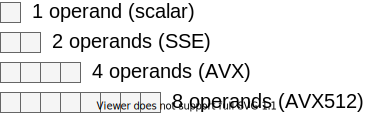
\includegraphics[width=\textwidth]{figures/registerwidth}

      \begin{challenge}{Challenge}
        Best code requires SIMD loads, stores, and arithmetic.
      \end{challenge}
    \end{column}
    \begin{column}{0.6\textwidth}
      \only<1>{Scalar addition, 1 output element per instruction.
        \begin{center}
          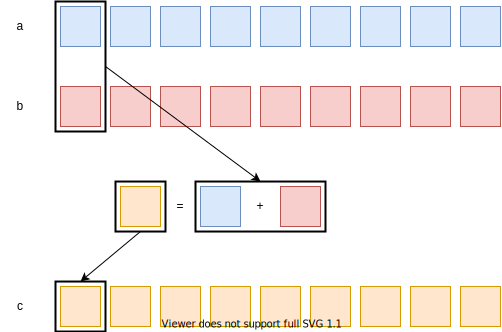
\includegraphics[width=0.9\textwidth]{figures/scalaradd}
        \end{center}}
      \only<2>{AVX addition, 4 output elements per instruction.
        \begin{center}
          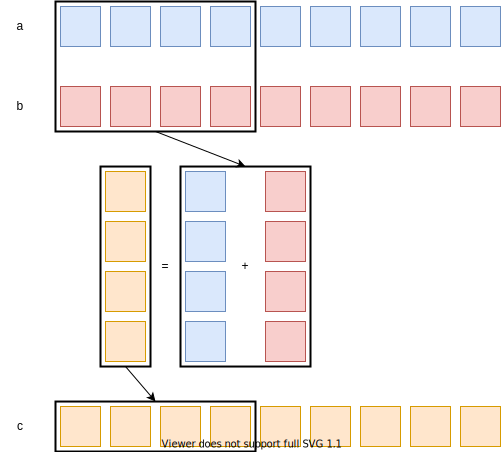
\includegraphics[width=0.9\textwidth]{figures/vectoradd}
        \end{center}}
    \end{column}
  \end{columns}
\end{frame}

\begin{frame}
  \frametitle{Data types in SIMD registers}
  Will focus on AVX (Advanced Vector eXtensions). 32-byte (256 bit)
  registers.

  \begin{center}
    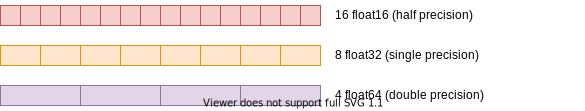
\includegraphics[width=\textwidth]{figures/vectorregisterdatatypes}
  \end{center}

  Machine learning is really excited about half precision because
  ``look how many numbers you can handle''.
\end{frame}

\begin{frame}[fragile]
  \frametitle{What does the compiler do?}
  \begin{exampleblock}{Unrolling}
    \vspace{0.5\baselineskip}
    \begin{columns}[t]
      \begin{column}{0.37\textwidth}
        Before
\begin{minted}{c}
for (i = 0; i < n; i++)
  c[i] = a[i] + b[i];
\end{minted}
      \end{column}
      \begin{column}{0.53\textwidth}
        After
\begin{minted}{c}
// Vectorisable loop
for (i = 0; i < n; i += 4) {
  c[i] = a[i] + b[i];
  c[i+1] = a[i+1] + b[i+1];
  c[i+2] = a[i+2] + b[i+2];
  c[i+3] = a[i+3] + b[i+3];
}
// Remainder loop
for (i = (n/4)*4; i < n; i++)
  c[i] = a[i] + b[i];
\end{minted}
      \end{column}
    \end{columns}
    \begin{center}
      {\large Don't do this by hand.}
    \end{center}
  \end{exampleblock}
\end{frame}

\begin{frame}[fragile]
  \frametitle{Roadblocks}
  \begin{challenge}{Carried dependencies}
    \begin{columns}
      \begin{column}{0.45\textwidth}
\begin{minted}{c}
for (i = 1; i < n; i++)
  c[i] = c[i] + c[i-1];
\end{minted}
        This has a \emph{loop carried dependency}.
      \end{column}
      \begin{column}{0.45\textwidth}
        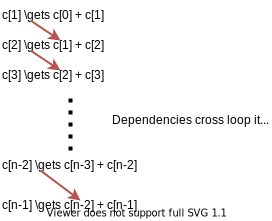
\includegraphics[width=\textwidth]{figures/loopcarrieddependency}
      \end{column}
    \end{columns}
  \end{challenge}
\end{frame}

\begin{frame}[fragile]
  \frametitle{Roadblocks}
  \begin{challenge}{Pointer aliasing (C/C++ only)}
\begin{minted}{c}
  void foo(double *a, double *b, double *c, int n) {
    for (int i = 0; i < n; i++)
      a[i] = b[i] + c[i];
  }
\end{minted}
  \end{challenge}
  \begin{exampleblock}{This is allowed}
\begin{minted}{c}
  void bar(double *data, int n) {
    double *a = data + 2;
    double *b = data + 1;
    double *c = data;
    // carried dependence in loop
    foo(a, b, c, n - 3);
  }
\end{minted}
  \end{exampleblock}
\end{frame}
\begin{frame}[fragile]
  \frametitle{Roadblocks}
  \begin{exampleblock}{This is allowed}
\begin{minted}{c}
  void bar(double *data, int n) {
    double *a = data + 2;
    double *b = data + 1;
    double *c = data;
    foo(a, b, c, n - 3);
  }
\end{minted}
  \end{exampleblock}
  \begin{center}
    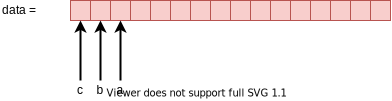
\includegraphics[height=0.3\textheight]{figures/pointeraliasing}
  \end{center}
\end{frame}

\begin{frame}[fragile]
  \frametitle{Pointer aliasing solution}
  \begin{challenge}{Pointer aliasing (C/C++ only)}
\begin{minted}{c}
  void foo(double *a, double *b, double *c, int n) {
    for (int i = 0; i < n; i++)
      a[i] = b[i] + c[i];
  }
\end{minted}
  \end{challenge}
  \begin{itemize}
  \item Smart compiler will ``multiversion'' this code. Check for
    aliasing and dispatch to appropriate version (expensive in hot
    loops).
  \item You can guarantee that pointers won't alias (C99 or better,
    not C++) with \texttt{restrict} keyword (\texttt{\_\_restrict\_\_}
    in many C++ compilers)
\begin{minted}{c}
  void foo(double * restrict a, double * restrict b,
           double * restrict c, int n)
\end{minted}
  \end{itemize}
\end{frame}

\begin{frame}[fragile]
  \frametitle{Options for generating SIMD code}
  \begin{answer}{In decreasing order of preference}
    \begin{enumerate}
    \item Compiler does it for you (but\dots)
    \item You tell the compiler what to do (directives)
    \item You choose a different (better) programming model. OpenCL,
      ispc
    \item You use \emph{intrinsics} (C/C++ only)
    \item You write assembly code
    \end{enumerate}
  \end{answer}

\begin{minted}[fontsize=\small]{c}
#include <x86intrin.h>
void foo(...) {
  for (j = 0; j < N; j += 8) {
    t0 = _mm_loadu_ps(data + j);
    t1 = _mm_loadu_ps(data + j + 4);
    s0 = _mm_loadu_ps(s0, t0);
    s1 = _mm_loadu_ps(s1, t1);
}
\end{minted}
\end{frame}

\begin{frame}
  \frametitle{Compiler options: Intel}
  \begin{itemize}
  \item At \texttt{-O2} or above, intel compiler will start
    vectorising
  \item Specific vector instruction sets can be selected with
    \texttt{-xFOO}
    \begin{enumerate}
    \item \texttt{-xSSE2} Everything post 2000ish

    \item \texttt{-xAVX} SandyBridge/IvyBridge (quite old)

    \item \texttt{-xCORE-AVX2} Haswell/Broadwell (somewhat old)
    \item \texttt{-xCORE-AVX512} Skylake/Icelake (pretty recent)
    \end{enumerate}
  \item Also prefer to set \texttt{-march=RELEVANTCPU},
    e.g.~\texttt{-march=broadwell}
  \item If you want AVX512 to really work, also need
    \texttt{-qopt-zmm-usage=high}
  \item Tell the compiler there are no pointer aliasing issues with
    \texttt{-fno-alias}. Don't lie here!
  \item See \texttt{icc -help} for more
  \end{itemize}
\end{frame}

\begin{frame}
  \frametitle{Compiler options: GCC}
  \begin{itemize}
  \item At \texttt{-O2} GCC vectorises if you also say
    \texttt{-ftree-vectorize} (or just use \texttt{-O3}).
  \item Specific instruction sets with
    \begin{itemize}
    \item \texttt{-msse2}
    \item \texttt{-mavx}

    \item \texttt{-mavx2} + \texttt{-mfma} (to enable FMAs)
    \item \texttt{-mavx512f}
    \item See \texttt{gcc --help-target} for more
    \end{itemize}
  \item Also prefer to set \texttt{-march=RELEVANTCPU},
    e.g.~\texttt{-march=broadwell}
  \item Provide a preferred vector width (in bits) with
    \texttt{-mprefer-vector-width=\{128,256,512\}}
  \item Tell the compiler there are no pointer aliasing issues with
    \texttt{-fargument-noalias}. Don't lie here!
  \end{itemize}
\end{frame}

\begin{frame}[fragile]
  \frametitle{How to know what is happening}
  \begin{itemize}
  \item Compilers can provide feedback on what they are doing
  \item Intel compiler is by \emph{far} the best here
  \item Enable output with \texttt{-qopt-report=n} ($n \in \{1, 2, 3,
    4, 5\}$) with larger values producing more detail
  \end{itemize}
\begin{exampleblock}{Example}
  \begin{columns}
    \begin{column}{0.3\textwidth}
\begin{minted}[fontsize=\scriptsize]{c}
 for (int i=1; i<n;i++)
   a[i] = a[i]+a[i-1];
\end{minted}
    \end{column}
    \begin{column}{0.6\textwidth}
\begin{minted}[fontsize=\scriptsize]{sh}
Begin optimization report for: foo(double *, int)
 Report from: Vector optimizations [vec]
LOOP BEGIN at <source>(6,3)
 remark #15344: loop was not vectorized:
   vector dependence prevents vectorization

 remark #15346: vector dependence: assumed
   FLOW dependence between a[i] (7:5)
        and a[i-1] (7:5)
LOOP END
\end{minted}
    \end{column}
  \end{columns}
\end{exampleblock}
\end{frame}

\begin{frame}[fragile]
  \frametitle{What if things aren't vectorised}
  \begin{itemize}
  \item Suppose you know that a particular loop is vectorisable, and
    should be, but the compiler just won't do it.
  \item[$\Rightarrow$] use OpenMP SIMD pragmas
  \item Turn on with \texttt{-qopenmp-simd} (Intel);
    \texttt{-fopenmp-simd} (GCC)
  \item Basic usage \texttt{\#pragma omp simd}
  \item Tells the compiler ``it's fine, please vectorise''
    $\Rightarrow$ don't lie!
    \begin{challenge}{Example}
      \begin{columns}
        \begin{column}{0.45\textwidth}
          Prerequisites
          \begin{itemize}
          \item Countable loop
          \item Inner loop
          \end{itemize}
        \end{column}
        \begin{column}{0.45\textwidth}
\begin{minted}{c}
for (j = 0; j < n; j++)
  #pragma omp simd
  for (i = 0; i < n; i++)
    b[j] += a[j*n + i];
\end{minted}
        \end{column}
      \end{columns}
    \end{challenge}
  \end{itemize}
\end{frame}

\begin{frame}[fragile]
  \frametitle{Overriding the compiler cost model}
  \begin{itemize}
  \item Compilers decide to do things based on some cost model
  \item[$\Rightarrow$] if the cost model is wrong, they may take
    ``bad'' decisions
  \item For vectorisation purposes we usually need to say ``please
    vectorise this loop'' or ``please unroll this loop''.
  \end{itemize}
  \begin{exampleblock}{Example}
    \vspace{0.5\baselineskip}
    \begin{columns}[t]
      \begin{column}{0.45\textwidth}
        Vectorisation
\begin{minted}{c}
#pragma omp simd
\end{minted}
      \end{column}
      \begin{column}{0.45\textwidth}
        Unrolling
\begin{minted}{c}
// Intel
#pragma unroll
#pragma unroll(n)
// GCC
#pragma GCC unroll(n)
\end{minted}
      \end{column}
    \end{columns}
  \end{exampleblock}
\end{frame}

\begin{frame}
  \frametitle{Exercise}
  \begin{itemize}
  \item What do you need to do to convince Intel compiler to vectorise the
    GEMM micro kernel?
  \item[$\Rightarrow$] Exercise 9.
  \end{itemize}
\end{frame}
\end{document}
